\chapter{Introduction}
- basic overview on the scope
\section{The LHC}
The Large Hadron Collider (LHC) at CERN is the largest particle collider in the world. It is located near Geneva in Switzerland and reaches into France with its 27\,km circumference. The LHC collides particles at an unprecedented center of mass energy ($\sqrt{s}$) of up to 13\,TeV and gives insight on the early stages of the universe. There are four major experiments, the ATLAS, ALICE, CMS, and the LHCb experiment, placed at four of the interaction points, where the opposing beams can be crossed (fig. \ref{fig:lhc_sketch}). There are three operation modes that are used regularly: pp, p--Pb, and Pb--Pb. Most of the time the LHC is operated with proton beams but usually one month per year either p--Pb or Pb--Pb collisions are performed. The first data was taken in RUN 1 in 2010 at $\sqrt{s}$\,=\,7\,TeV. This run lasted until early 2013 when the first long shutdown took place to upgrade the LHC in order to increase the collision energy. RUN 2 started with $\sqrt{s}$\,=\,13\,TeV in June 2015 and is planned to be concluded by the end of 2018. Then, the second long shutdown will proceed, featuring major upgrades to the LHC to increase its luminosity.\\
The purpose of the LHC is to allow for the testing of theories and predictions in nuclear and particle physics. Therefore, physicists try to find new particles, as successfully done with the Higgs Boson. In addition, a new state of matter is sought after -- the quark-gluon plasma. 

\begin{figure}[]
	%\begin{minipage}[c]{\textwidth}
		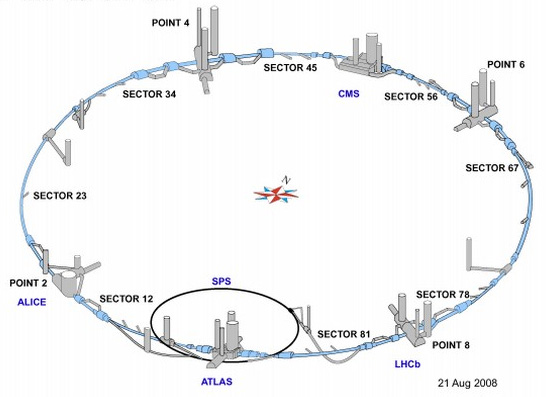
\includegraphics[width=\textwidth]{pictures/lhc.jpg}
	%\end{minipage}\hfill
	%\begin{minipage}[c]{\textwidth}
		\caption{Sketch of the LHC (light blue) with the four major experiments.}
		\label{fig:lhc_sketch}
	%\end{minipage}
\end{figure}


\section{The ALICE detector}
ALICE (A Large Ion Collider Experiment) is one of the four major detectors at the LHC ring. This heavy ion detector is built to study the physics of strong interacting matter in extreme conditions. \\
In ordinary matter, quarks occur either in pairs or triplets to form mesons and hadrons. However, single quarks are never observed since they are bound by gluons and confined inside compound particles. This phenomenon is known as confinement. In the extreme temperatures generated in Pb--Pb collisions, which reach up to 100'000 times the temperature of the Sun's centre, a new state of matter has been predicted -- the quark-gluon plasma. In this hot and dense state particles "melt" and the quarks are deconfined. Similar conditions were present just after the big bang. By recreating the quark-gluon plasma in the laboratory we are able to study the evolution of the early universe and the hadronisation process that lead to the creation of ordinary matter as we know it in today's universe. The ALICE detector was build to do exactly that: study the quark-gluon plasma and ,therefore, the origin of our existence.\\
\begin{figure}[]
	%\begin{minipage}[c]{\textwidth}
		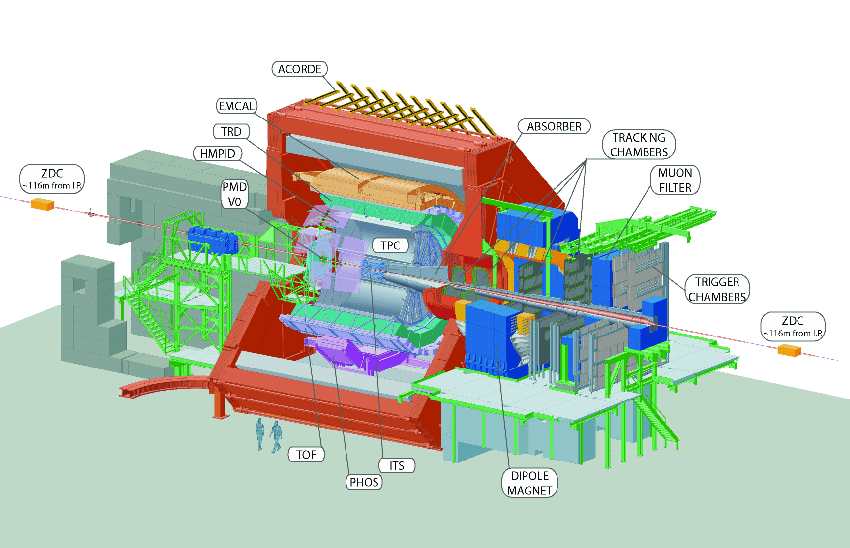
\includegraphics[width=\textwidth]{pictures/The-ALICE-Detector-Figure-taken-from-6.png}
	%\end{minipage}\hfill
	%\begin{minipage}[c]{\textwidth}
		\caption{The ALICE detector [source: The ALICE experiment at the CERN LHC (JINST)].}
		\label{fig:ALICE_sketch}
	%\end{minipage}
\end{figure}
The detector consists of a variety of sub-detectors allowing for the detection of hadrons, electrons, muons, and photons produced in heavy ion collisions (fig. \ref{fig:ALICE_sketch}). There are central detectors covering the interaction point around mid-rapidity ($\eta$\,=\,0), the muon spectrometer at -4\,<\,$\eta$\,<-2.5, and forward detectors covering high $\vert\eta\vert$ regions. The different parts of ALICE combine to a machine that is capable of identifying and tracking the particles arising from the collision. This work focuses on the TPC, one of the central detectors.
%\subsection{Particle detection in ALICE}
%\subsection{Advantages and restrictions}
\section{Opportunities in RUN 3}
- upgrade to HL-LHC

- difference to previous runs

- what can be done with more data? -> opportunities
\section{A new software framework -- O\textsuperscript{2}}
- DAQ and analysis framework ALIROOT

- new challenges with continuous readout

- new framework O2 with its advantages